\section{Introduction}
\label{sec:introduction}

% \begin{figure}[t]
%     \includegraphics[width=\linewidth]{images/introduction_problem_3.pdf}
% \caption{Decomposition of a user request into sub-queries with associated retrieved documents. In a RAG setting, these documents serve as evidence of information and are used to generate a grounded answer. We formulate this as a problem of exploration (more sub-queries) and exploitation (more documents per sub-query) problem and use bandit learning methods to dynamically determine the right balance.}
%     \label{fig:query_decomposition_task}
% \end{figure}

%% Introduction of problem
Complex user queries usually involve discourse operators such as the exclusion of information \cite{excluir}, negation \cite{petcu2025comprehensivetaxonomynegationnlp, nevir, repro_nevir}, or missing entities \cite{reasoning_missing_entities, tip_of_the_tongue}, and often require retrieving evidence found in multiple documents.
%Traditional lexical models for addressing complex queries are limited to keyword matching. Dense retrieval models attempt to create one contextual representation for the entire query and retrieve documents that match this representation globally \cite{dense_better, dense_better_2}. However, dense methods often fail to account for the logical structures of complex queries, where different components may correspond to different sources of information scattered throughout the corpus. 
%% RAG and deocomposition
One way to handle them is to decompose the request into atomic sub-queries~\cite{khot2023decomposedpromptingmodularapproach}, as shown in Figure~\ref{fig:query_decomposition_task}. %A retrieval-augmented generation (RAG) \cite{lewis2021retrievalaugmentedgenerationknowledgeintensivenlp} pipeline can then retrieve documents independently for each sub-query, reason over and aggregate the information into one coherent, grounded answer.
%% Motivation
Retrieving documents independently for each sub-query leads to coverage of complex information needs by maximizing recall. However, it may result in a large number of documents, of which many are irrelevant \cite{kim2025NotInformative}. This is problematic in two ways. 
First, too many documents cannot fit in the context window of an LLM, without being arbitrarily truncated, potentially removing vital information.
Second, including a large proportion of irrelevant documents introduces noise in the generation \cite{jin2024longcontextllmsmeetrag}. 
Mitigating these problems involves filtering by either human annotators or LLM agents. This motivates our core question: \emph{how to efficiently identify which sub-queries are likely to retrieve relevant information and what constitutes an appropriate retrieval depth for each sub-query}?

\begin{figure*}[t]
    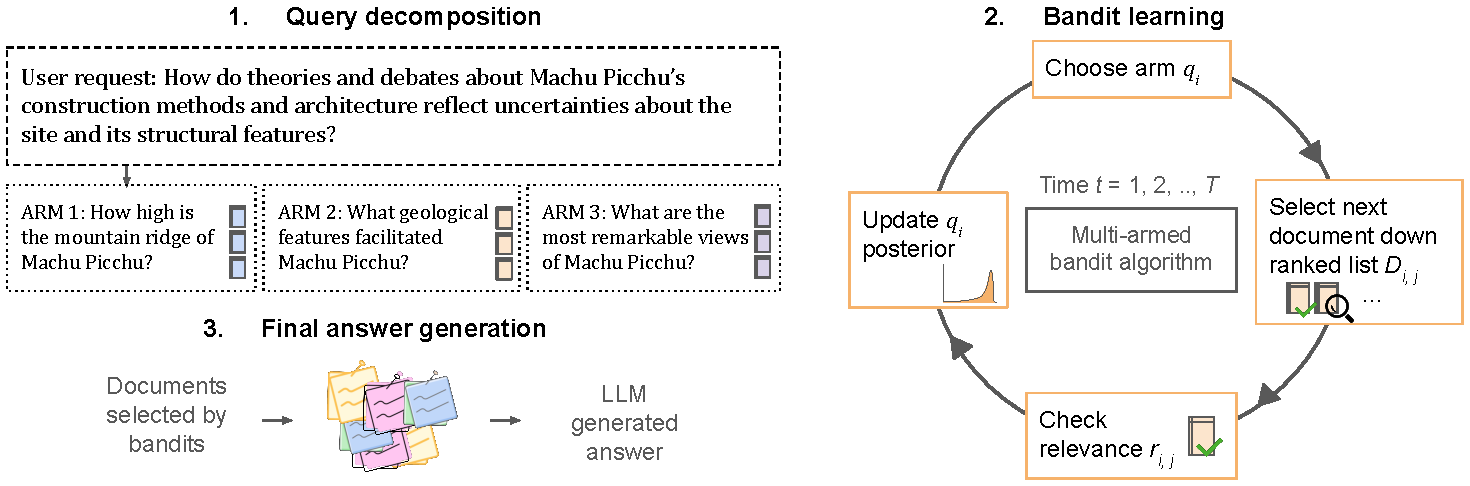
\includegraphics[width=\linewidth]{images/introduction_problem_10.pdf}
\caption{A user request is first decomposed into sub-queries. Bandit learning iteratively selects a sub-query (arm), retrieves a document down its ranked list, observes its relevance, and updates the sub-query posterior belief over time. The selected documents across iterations are then used as evidence in a RAG setting to generate a grounded answer, balancing exploration (more sub-queries) and exploitation (more documents per sub-query).}
    \label{fig:query_decomposition_task}
\end{figure*}

%% Gap in Research
Existing approaches to sub-query decomposition and document retrieval lack a principled mechanism for allocating documents, with most methods retrieving a fixed number of documents regardless of sub-query utility. Meanwhile, we want to study a method that adaptively decides, under a fixed budget, whether to continue retrieving documents from an observed, promising sub-query or to explore alternatives that may yield more relevant evidence, while avoiding irrelevant overlap. A multi-armed bandit framework naturally captures this process: each sub-query is treated as an arm, for which each observed document provides evidence of its utility.
%We propose modeling the problem of query decomposition and document retrieval in an exploration-exploitation setting and using multi-armed bandit learning to make informative decisions on which sub-query, and to which extent each sub-query is relevant to the user information need. 
%% Options
% Query decomposition offers a straightforward way to address complex information needs by breaking down the user request into multiple sub-queries. To maximize recall, one might generate a large number of sub-queries for which a system retrieves an extensive pool of documents. However, this strategy results in a large amount of documents that are irrelevant for the user request \cite{kim2025NotInformative} and can ultimately harm downstream performance. One option to mitigate this issue is to assess document relevance using large language model (LLM) judges, using their parametric knowledge and in-context learning capabilities. %However, this approach is expensive and not fully reliable, as each LLM call adds noise by possibly lacking factual grounding, particularly in cases where a query answer cannot straightforwardly be found in a small amount of documents. 
% Another option is to use humans-in-the-loop as domain-expert annotators. Both approaches come with the disadvantages of being expensive in effort overload, financial and time resources, making them difficult to scale in practice. 
Framing query decomposition and document selection as a bandit problem  addresses two core challenges of complex information needs. First, retrieval is inherently sequential and budget-constrained, as it is impossible to verify all documents. Second, the relevance of a sub-query is initially uncertain, while our belief of its relevance builds with each retrieved document.


Figure \ref{fig:query_decomposition_task} illustrates our setting. We estimate the utility of each sub-query, modeled as an arm, by observing the relevance of one document at a time. The choice of assessment directly influences the cost. By estimating utility under a fixed budget, i.e., at each step the system makes a choice between going down the ranked list of a certain sub-query or retrieving from a new one, the process becomes considerably more efficient. This perspective is complementary to recent approaches on efficient selection under computational constraints, such as compute-efficient re-ranking \citep{SetwiseInsertion2024} and training data selection \citep{petcu2024efficientdataselectionemploying}. In the example shown in Figure \ref{fig:query_decomposition_task} %, the algorithm chooses the second sub-query, selects the next documents down its ranked list, and uses its relevance to update a belief about its utility. In this setting, 
we assume access to a user request, its decomposition, document relevance (assessed by either LLM judges or human annotators), and a search engine %through which we retrieve documents. Given a limited budget of documents, 
We aim to answer the following research questions:


%Figure \ref{fig:tradeoff} shows a cost comparison between our proposed method, and using either LLM judges or human annotators. We assume access to a user request that is split into a large number of sub-queries \cite{Verma2024PlanRAGETA, Cai2024MixGRERA}, which we model as the arms in our bandit learning setting.  We also assume that each sub-query can be used as input to a search engine to retrieve relevant documents. Given a limited budget of documents we can retrieve and assuming that we can only observe/evaluate one document at a time, we aim to answer the following research questions:


% \begin{figure}[!h] 
% 	\centering
% 	\includegraphics[width=\linewidth]{images/tradeoff-cost.png}
% 	\caption{Cost trade-off between bandit learning, llm judges and human assessment. The cost has been calculated using the following data: (1) we consider using gpt-4o with a pricing of 2.5 USD per 1M input tokens; considering the token limit of 128 tokens as one document; (2) for humans we consider the same document length of 128k tokens, corresponding to approximately 100k words that takes around 6h of reading by an experienced assessor; (3) for bandit learning, the only cost comes from I/O}
% 	\label{fig:tradeoff}
% \end{figure}

% \begin{figure}[!t] 
% 	\centering
% 	\includegraphics[width=\linewidth]{images/bandits_costs.pdf}
% 	\caption{Cost trade-off between bandit learning, LLM judges and human assessment. The cost has been calculated using the following data: (i) we consider using GPT-4o with a pricing of 2.5 USD per 1M input tokens; considering the token limit of 128 tokens as one document; (ii) for humans we consider the same document length of 128k tokens, corresponding to approximately 100k words that takes around 6h of reading by an experienced assessor; (iii) for bandit learning, the only cost comes from I/O.}
% 	\label{fig:tradeoff}
% \end{figure}

\begin{enumerate}[label=(RQ\arabic*),leftmargin=*,nosep]
    \item How can query selection be framed as a multi-armed bandit problem? Does bandit learning outperform full exploitation and full exploration strategies? What strategies best balance exploration with exploitation?
    \item Does document selection using multi-armed bandits improve evaluation metrics on the downstream task of report generation?
    \item Can bandit learning be used to guide hierarchical sub-query decomposition?
\end{enumerate}

\noindent%
For answering RQ1, we model query decomposition and document retrieval in an efficient way using reinforcement learning (RL) policies in a multi-armed bandit setting, demonstrating that estimating Bernoulli distributions boosts relevance estimates by \(17\%\) compared to simply going down the ranked list. With RQ2, we look into the performance of using an optimal subset of documents for report generation, in which we improve on evaluation metrics such as nugget coverage and sentence support. With RQ3, we examine the use of hierarchical, multi-level sub-query decomposition, which yields a \(30\%\) precision gain over selecting all documents from a single-level decomposition.